\section{Main Algorithm}\label{sec:algo}

To address these problems, we extended \learnpads{} to work
incrementally.  
\figref{fig:overview} illustrates a high level schematic of this
algorithm. 
Given a candidate description \cd{D}, the new algorithm uses \cd{D} to parse
the records in the data source.  
It discards records that parse successfully, since these records are
already covered by \cd{D}, but it collects records that fail to parse.
When the algorithm accumulates $M$ such records, where $M$ is a
parameter of the algorithm, it invokes the incremental learning step,
described below, to produce a refined description \cd{D'}.  This refined
description subsumes \cd{D} and describes the $M$
new records.  In addition, the algorithm attempts to preserve as much
of the structure of \cd{D} as possible, so users supplying initial
descriptions can recognize the resulting descriptions. 
The algorithm then takes \cd{D'}
to be the new candidate description and repeats the process until it
has consumed all the input data.
The initial description \cd{D} can either be supplied by a user or it
can be inferred automatically by applying the original algorithm to
$N$ records selected from the data source, where $N$ is another
parameter.  
%Currently, the system selects a mix of $N/3$ consecutive lines
%taken from the beginning, middle, and end of the data source. 


Intuitively, the incremental learning step works by attempting to
parse each of the $M$ records according to the current description
\cd{D}.  It discards the portions of each record that parse correctly.
If a portion fails to parse, that failure will be detected at a
particular node in the description \cd{D}. It collects these failed
portions in an aggregation data structure \cd{A} that mirrors the
structure of \cd{D}.  After thus aggregating all the failures in the $M$
records, the algorithm transforms \cd{D} to accommodate the places where
differences were found (\ie, by introducing options where a piece of
data was missing or unions where a new type of data was discovered).
It then uses the original \learnpads{} algorithm to infer descriptions
for the aggregated portions of bad data. 

\cut{
Intuitively, the incremental learning algorithm takes an initial
description as input, divides the new data into manageable
chunks, and iteratively merges descriptions of these chunks into the
current description.
\figref{fig:overview} illustrates a high level schematic of this
algorithm. A large or streaming data source is input 
to the system in batches. Each batch of data contains $M$ 
records, where $M$ is a parameter of the framework.
%%The state of the system is determined by the current data
%%description which is subject to change as new data streams into the system. 
The initial description
can be supplied by user, or learned from the first batch of the input
data. At each iteration, the system generates a filter program from
the current data description.  This program parses the incoming batch of data
into an aggregted data structure similar to the parse tree of the description.
In this process, the filter program collects ``bad data'' which does not
comform to the current description. The system then invokes the original
\learnpads{} algorithm to learn ``sub-descriptions'' from the bad data, and
merges these sub-descriptions into the current data description to produce
a new description for the next iteration. 
}
\begin{figure}[th]
\centering
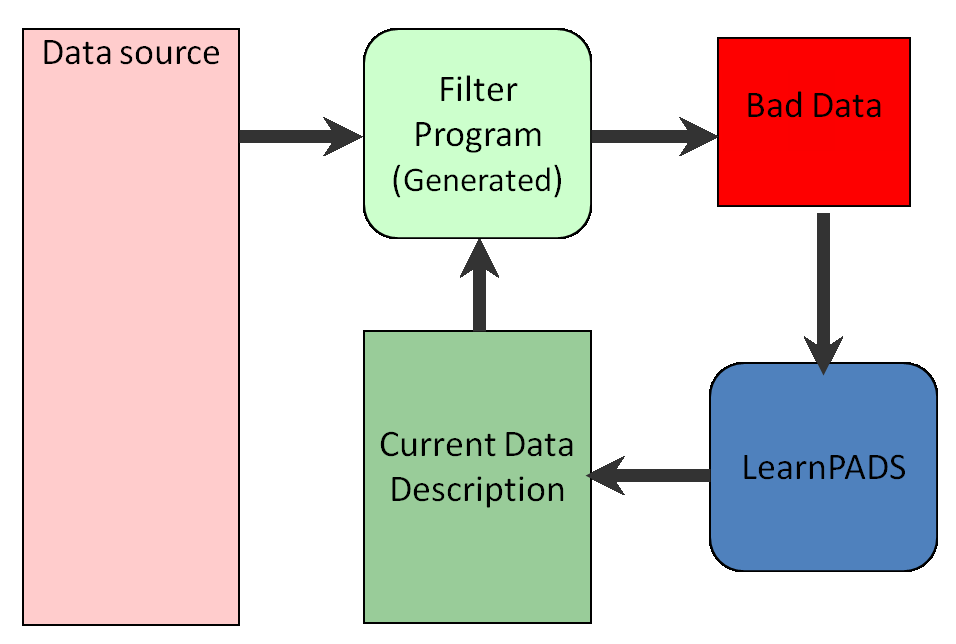
\includegraphics[width=0.9\columnwidth]{overview}
%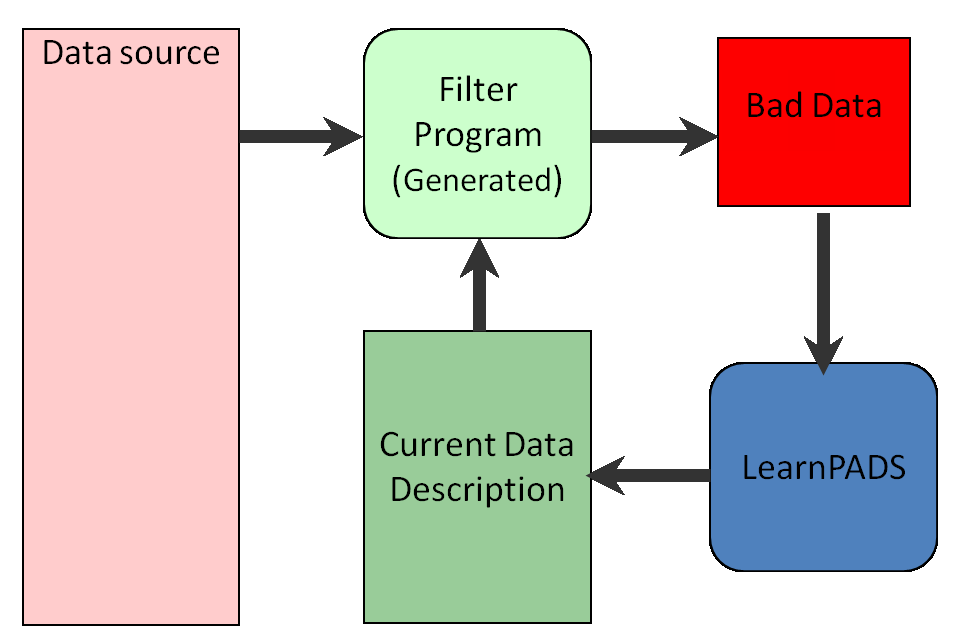
\epsfig{file=overview.eps,width=0.9\columnwidth}
\caption{An Overview of the Incremental Learning Framework}
\label{fig:overview}
\end{figure}

In the rest of this section, define we some preliminary data
structures and then present the algorithm in more detail, giving the
operational semantics of two key functions ({\em parse} and {\em
  aggregate}) and describing some optimizations to refine the
description learned in each step.

%To address these problems, 
%we extended \learnpads{} to work incrementally.  
%Given a candidate description \cd{D}, the new algorithm uses \cd{D} to parse
%the records in the data source.  
%It discards records that parse successfully, since these records are
%already covered by \cd{D}, but it collects records that fail to parse.
%When the algorithm accumulates $M$ such records, where $M$ is a
%parameter of the algorithm, it invokes the incremental learning step,
%described below, to produce a refined description \cd{D'}.  This refined
%description subsumes \cd{D} and describes the $M$
%new records.  In addition, the algorithm attempts to preserve as much
%of the structure of \cd{D} as possible, so users supplying initial
%descriptions can recognize the resulting descriptions. 
%The algorithm then takes \cd{D'}
%to be the new candidate description and repeats the process until it
%has consumed all the input data.
%The initial description \cd{D} can either be supplied by a user or it
%can be inferred automatically by applying the original algorithm to
%$N$ records selected from the data source, where $N$ is another
%parameter.  
%Currently, the system selects a mix of $N/3$ consecutive lines
%taken from the beginning, middle, and end of the data source. 

\subsection{Preliminaries}

\begin{figure}[t]
{\small 
\begin{code}
\kw{Basic notations}:
c          (a string character)	
s1.s2      (concatenation of strings)
prefix(s)  (set of prefixes of s)
sprefix(s) (set of strict prefixes of s)
\end{code}
\begin{code}
\kw{Descriptions}:
Base ::= Pint | PstringME(re) | PstringFW(e)
\end{code}
\begin{code}
D ::=   
  Base               (Base token)
| Sync s             (Synchronizing token) 
| Pair (x:D1, D2)    (Pair with dependency)
| Union (D1, D2)     (Union)
| Array(D, s, t)     (Array)
| Option D           (Option)
\end{code}
\begin{code}
\kw{Data representation}:
BaseR ::= Str s | Int i | Error
\end{code}
\begin{code}
SyncR ::= Good | Fail | Recovered s 
\end{code}
\begin{code}
R ::=
  BaseR
| SyncR
| PairR (R1, R2)
| Union1R R | Union2R R 
| ArrayR (R list, SyncR list, SyncR)
| OptionR (R option)
\end{code}
\begin{code}
\kw{Aggregation structure}:
A :: = 
  BaseA Base
| SyncA s
| PairA(A1, A2)
| UnionA(Al, Ar)
| ArrayA (A_elem, A_sep, A_term)
| OptionA A
| Opt A
| Learn [s]
\end{code}
}
\caption{Preliminary data structures used in incremental inference}
\label{fig:data-structures}
\end{figure}

\cut{%%%%%%%%%%%%%%%%%%%%%%%%%%%%%%%%%%%%%%%%%
Intuitively, the incremental learning step works by attempting to
parse each of the $M$ records according to the current description
\cd{D}.  It discards the portions of each record that parse correctly.
If a portion fails to parse, that failure will be detected at a
particular node in the description \cd{D}. It collects these failed
portions in an aggregation data structure \cd{A} that mirrors the
structure of \cd{D}.  After thus aggregating all the failures in the $M$
records, the algorithm transforms \cd{D} to accommodate the places where
differences were found (\ie, by introducing options where a piece of
data was missing or unions where a new type of data was discovered).
It then uses the original \learnpads{} algorithm to infer descriptions
for the aggregated portions of bad data. 
}%%%%%%%%%%%%%%%%%%%%%%%%%%%%%%%%%%%%%%%%%%%%%%%%%%%%

\figref{fig:data-structures} defines
the data structures for descriptions \cd{D}, data
representations \cd{R}, and aggregate structures \cd{A}.
In these definitions,  variable \cd{re} ranges over regular expressions,
\cd{e} over host language expressions,
\cd{s} and \cd{t} over strings, and \cd{i} over integers.
A value with type \cd{D} is the abstract syntax tree of \pads{}
description: this description is what we want to learn.  
For simplicity of presentation, we assume just three base types: 
integers, strings that match a regular expression and strings with a
fixed width specified by an expression. Synchronizing
tokens, or {\em sync tokens} for short, correspond to string literals
in \pads{} descriptions.  Such tokens, which are often
white spaces or punctuation,
serve as delimiters in the data and are useful for detecting
errors. We use binary dependent pairs \cd{Pair (x:D1, D2)} to model \kw{Pstruct}s. 
The variable \cd{x} is bound in the second component of the
pair to the value in the first componenet.
We use  unions to account for \kw{Punion}s. 
An array \cd{Array(D, s, t)} has an element type described by \cd{D}, a separator
string \cd{s} that appears between array elements, and a
terminator string \cd{t}. \cd{Option D} indicates \cd{D} is optional.

A term with type \cd{R} is a parse tree obtained from parsing 
data using a description \cd{D}.  Parsing a base type can result in a
string, an integer or an error.  Parsing a sync token
\cd{Sync s} can give three different results: \cd{Good}, meaning the
parser found \cd{s} at the beginning of the input; \cd{Fail}, meaning
\cd{s} is not a substring of the current input; or \cd{Recovered s'},
meaning \cd{s} is not found at the beginning of the input, but
can be {\em recovered} after ``skipping'' string \cd{s'}.  The parse
of a pair is a pair of representations, and the parse of a union is
either the parse of the first branch or the parse of the second
branch. The parse of an option is either the parse of its body or  empty.
The parse of an array includes a list of parses for the
element type, a list of parses for the separator and a parse for the
terminator which appears at the end of the array.

An aggregation structure is the {\em accumulation} of parse trees; it
collects the data that cannot be parsed (in other words, error data)
and therefore must be re-learned.
The aggregation structure mirrors the structure of the description \cd{D} 
with two additional nodes: an \cd{Opt} node and a \cd{Learn} node. 
An invariant is that an \cd{Opt} node always wraps a \cd{BaseA} or a \cd{SyncA} node,
where it indicates that the underlying base or sync token is missing
in some of the parses being aggregated, and therefore that the wrapped
token should be made optional. 
%Note the difference between {\tt Opt} nodes and {\tt OptionA} nodes. The latter 
%just corresponds to the description {\tt Option D}. 
The \cd{Learn} node accumulates the bad portions of the data.
Once the system infers a description for this accumulated data, it
splices in the new description in place of the \cd{Learn} node.

\subsection{Incremental Learning Step}
\begin{figure}[t]
\begin{codebox}
incremental_step(d, xs) =
  as = [\kw{init_aggregate}(d)];
  foreach x in xs \{
    rs = \kw{parse}(d, x);
    as' = [];
    foreach r in rs \{
      foreach a in as \{
        a' = \kw{aggregate}(a, r); 
        as' = a :: as'
      \}
    \}
    as = as'
  \} 
  best_a = \kw{select_best}(as);
  d' = \kw{update_desc}(d, best_a);  
  return d'
\end{codebox}
\caption{Pseudo-code for the incremental learning step}
\label{fig:inc-learning}
\end{figure}

\figref{fig:inc-learning} gives pseudo-code for the {\em incremental
  learning step}.  The input to this step is the current description
\cd{d} and a batch of data records \cd{xs}.  The \cd{init\_aggregate}
function initializes an empty aggregate according to description
\cd{d}.  During parsing, the algorithm iteratively updates a list of
possible aggregates \cd{as}, seeded with the initial aggregate of
\cd{d}.  For each data record \cd{x}, the algorithm uses the
\cd{parse} function to produce a list \cd{rs} of possible parses.  It
then calls the \cd{aggregate} function to merge each parse \cd{r} in
the current list of parses with each aggregate \cd{a} in the current
list of aggregates.  (We use `\cd{::}' to denote prepending an element
onto the front of a list.)  When the system finishes parsing all the
input data, the algorithm uses the \cd{select\_best} function to
select the best aggregate from the list of candidate aggregates
\cd{as}.  The \cd{select\_best} function counts the total number of
\cd{Opt} and \cd{Learn} nodes in each of the aggregates, and returns
the one with the smallest number.
The idea is that the aggregate with the smallest number of added nodes is 
more likely to represent a new description
that is the closer to the original description. 
Finally, the \cd{update\_desc} function uses the structure of the best
aggregate to update the previous description \cd{d} to produce the new
current description \cd{d'}.  The \cd{update\_desc} function works by
doing two things.
First, it converts the aggregate structure back to a \pads{} description
with \cd{Opt} nodes translated to \cd{Poption} types. In addition,
it invokes the \learnpads{} format inference
algorithm to learn a sub-description for the data collected 
at each of the \cd{Learn} nodes
and replaces these \cd{Learn} nodes with these new sub-descriptions. 
Second, it uses rewriting
rules into improve the overall structure.
We will discuss these rewriting rules in more
detail in \secref{sec:imp}.

\begin{figure}[t]
%\begin{center}
{\small
\begin{code}
\cdmath\small
\kw{Base}:
(Int (atoi s), m) $\in$ L(Pint,E,s,s')
  if m = (0,0,len(s))
(Error, (1,0,0)) $\in$ L(Pint,E,"",s'), 
  if s $\in$ L((+|-)?[0-9]+) 
  and L([0-9]) $\cap$ prefix(s') = \{\}
(Str s, m) $\in$ L(PstringME(re),E,s,s'),
  if s $\in$ L(re) 
  and m = (0,0,len(s)) 
  and s.s'' $\not\in$ L(re) and s'' $\in$ prefix(s') 
(Error, m) $\in$ L(PstringME(re),E,"",s'), 
  if "" $\not\in$ L(re)
  and m = (1,0,0)
(Str s, m) $\in$ L(PstringFW(e),E,s,s') 
  if E(e) = Int k and s = c1...ck
  and m = (0,0,len(s))
(Error, (1,0,0)) $\in$ L(PstringFW(e),E,"",s') 
  if E(e) $\ne$ Int k for any k
(Error, (1,0,0)) $\in$ L(PstringFW(e),E,"",s') 
  if E(e) = Int k and k > 0
\mbox{}
\kw{Sync}:
(Good, (0,0,len(s))) $\in$ L(Sync(s),E,s,s')
(Recovered s1, m) $\in$ L(Sync(s2),E,s,s')
  if s=s1.s2 and s2 $\not\in$ prefix(s1.s2)
  and m = (1,len(s1),len(s2))
(Fail, (1,0,0)) $\in$ L(Sync(s2),E,"",s')
\mbox{}
\kw{Pair}:
(PairR (R1,R2), (m1 + m2)) 
        $\in$ L(Pair(x:D1, D2),E,s1.s2,s')
  if  (R1, m1) $\in$ L(D1,E,s1,s2.s')
  and (R2, m2) $\in$ L(D2,E[x $\arrow$ R1],s2,s')
\mbox{}
\kw{Union}:
(Union1R R, m) $\in$ L(Union(D1, D2),E,s,s')
  if (R, m) $\in$ L(D1, E, s, s')
(Union2R R, m) $\in$ L(Union(D1, D2),E,s,s')
  if (R, m) $\in$ L(D2, E, s, s')
\mbox{}
\kw{Main parse function}:
\kw{parse}(D, s) = \{R | (R, m) $\in$ L(D,.,s,"")\} 
\end{code}
%and for all (R',m') $\in$ L(D,.,s,""), m <= m'
}
\caption{Semantics of parsing (selected elements)}
\label{fig:parse-sem}
%\end{center}
\end{figure}

%% \kw{Array}:
%%   (ArrayR([R1,...,Rn], [SyncR1,...,SyncR(n-1)], $SyncR_{term}$), m)
%%     $\in$ L(Array(D, $s_{sep}$, $s_{term}$), E, s, s'),
%%         if
%%         s = s1.$s_{sep}$.s2.$s_{sep}$...s(n-1).$s_{sep}$.sn,
%%         lookaheadfori = $s_{sep}$.s(i+1).....sn.s'
%%         lookaheadforsepi = s(i+1)....sn.s'
%%         s' = s1'.lookaheadforterm

%%         forall i $\in$ [1, n]:
%%           (Ri, mi) $\in$ L(D, E, si, lookaheadfori),
%%         forall i $\in$ [1, n-1]:
%%           (SyncRi, m(s,i)) $\in$ L(Sync($s_{sep}$), E, $s_{(sep,i)}$, lookaheadforsepi),

%%         ($SyncR_{term}$, $m_{term}$) $\in$ L(Sync($s_{term}$), E, s1', lookaheadforterm),
%%         m = $\sum_{i= 1}^{n} mi$ + $\sum_{i=1}^{n-1} m(s,i)$ + $m_{term}$
%% \mbox{}
%% \kw{Option}:
%% (OptionR (SOME R), m) $\in$ L(Option D, E, s, s')
%%   if (R, m) $\in$ L(D, E, s, s')
%% (OptionR (NONE), m) $\in$ L(Option D, E, "", s')
%%   if (R, m) $\in$ L(D, E, "", s')



\subsection{The parse function}
\label{sec:parse}
To define the \cd{parse} function, we first introduce some useful notation.
An {\em environment} is a mapping between variable names and parses.
\[E : x \arrow R \]

A {\em parse metric} $m$ measures the quality of a parse. It is a 
triple: ($e$, $s$, $c$), where the $e$ is the number of tokens
with parse errors, $s$ is the number of 
characters skipped during \cd{Sync} token recovery, 
and $c$ is the number of characters correctly parsed. 
The following formulas define addition and inequality for parse metrics:
\begin{eqnarray}
&&(e1, s1, c1) + (e2, s2, c2) = (e1 + e2, s1 + s2, c1 + c2)  \\ 
&&(e1, s1, c1) \ge (  e2, s2, c2)~ \rm{iff}~ \frac{c_1}{s_1+c_1} 
\ge \frac{c_2}{s_2 + c_2} \label{eqn:metric-eqn}
\end{eqnarray}

To facilitate the presentation of \cd{parse}, we define the judgement:
\[(R, m) \in L(D, E, s, s')\]
which can be read ``with an environment $E$, a description $D$
can be parsed into $R$ with a metric $m$, while consuming
string $s$, with a lookhead string $s'$ that remains unconsumed''.
\figref{fig:parse-sem} gives the full semantics of this judgement and
the definition of \cd{parse} that uses this judgement.

\subsection{The aggregate function}
\begin{figure}[t]
\centering
\begin{code}
\cdmath
\kw{Opt a : Opt [Base]}:
  Opt a + Error $\goto$ Opt a
  Opt a + b     $\goto$ Opt b::a
\mbox{}
\kw{a : [Base]}:
  a + Error $\goto$ Opt a
  a + b     $\goto$ b::a
\mbox{}
\kw{a : [Sync s]}: 
  a + Good $\goto$ Good :: a
  a + Fail $\goto$ Opt a
  a + Recovered s' $\goto$ (Opt(l [s'], Good :: a)
\mbox{}
\kw{Opt a : Opt [Sync s]}: 
  Opt a + Good $\goto$ Opt (Good :: a)
  Opt a + Fail $\goto$ Opt a
  Opt a + Recovered s' $\goto$ 
    (Opt (l [s]), Opt (Good :: a))
\mbox{}
\kw{(Opt(l Ss), a) : Opt L * [Sync s]}:
  (Opt(l Ss), a) + Good $\goto$ 
    (Opt(l Ss), Good :: a)
  (Opt(l Ss), Opt a) + Fail $\goto$ 
    (Opt(l Ss), Opt a)
  (Opt(l Ss), Opt a) + Recovered s' $\goto$ 
    (Opt(l s':: Ss), Opt Good :: a)
\mbox{}
\kw{Pair(x:D1, D2)}:
  PairA($a_1$, $a_2$) + PairR($r_1$, $r_2$) $\goto$ 
    PairA($a_1\prime$, $a_2\prime$),
    if  $a_1 + r_1 \goto a_1\prime$
    and $a_2 + r_2 \goto a_2\prime$
\mbox{}
\kw{Union(D1, D2)}:
  UnionA($a_l$, $a_r$) + Union1R $r_l \goto$ 
    UnionA($a_l\prime$, $a_r$)
    if $a_l + r_l \goto a_l\prime$
  UnionA($a_l$, $a_r$) + Union2R $r_r \goto$ 
    UnionA($a_l$, $a_r\prime$)
    if $a_r + r_r \goto a_r\prime$
\end{code}
\caption{Semantics of aggregation (selected elements)}
\label{fig:aggr-sem}
\end{figure}

%% \kw{Array(D, $D_{sep}$, $D_{term}$)}:
%%   ArrayA($a_e, a_s, a_t$) + ArrayR(elems, seps, term) $\goto$ array($a_e\prime, a_s\prime, a_t\prime$)
%%   if 
%% 	$a_e$ ++ elems $\goto a_e\prime$
%% 	$a_s$ ++ seps  $\goto a_s\prime$
%% 	$a_t$ +  term  $\goto a_t\prime$

%% \kw{Option D}:
%%   OptionA a + OptionR (SOME r) $\goto$ OptionA a' if a + r $\goto$ a'
%%   OptionA a + OptionR (NONE) $\goto$ OptionA a 

%% \kw{Aggregation of list}:
%%   a ++ [] $\goto$ a

%%   a ++ (r :: rs) $\goto$ a'' 
%%   if 
%% 	a + r $\goto$ a'
%% 	a ++ rs $\goto$ a''


\figref{fig:aggr-sem} gives the definition of the \cd{aggregate}
function.
In the figure, $a$ and $b$ range over aggregate structures, while
$r$ ranges over data representations, \ie{} parses.
We use two judgement forms to define the \cd{aggregate} function:
\[A + R \goto A'\]
represents aggregate $A$ plus a data representation $R$ rewrites to $A'$.
This corresponds to the \cd{aggregate} function.
\[A ++ Rs \goto A'\]
represents aggregate $A$ plus a list of representations $Rs$ rewrites
to $A'$. This is used in the aggregation of arrays.


\subsection{Examples}
To illustrate the parsing and aggregation phases of the algorithm, we
introduce a simple example.
Suppose we have a description $d$, comprised of a pair of an integer and a sync token ``\cd{*}'',
and we are given the following three lines of new input:

{\small \texttt{
\begin{tabular}{l}
5*\\
abc*\\
8\$\\[1ex]
\end{tabular}}
}

\noindent
\figref{fig:parse} shows the three data representations that result
from parsing the lines, which we call $r_1$, $r_2$ and $r_3$,
respectively. Notice the first line parsed without errors, the second
line contains an error for \cd{Pint} and some unparsable data ``{\tt
  abc}'', and the third contains a \cd{Fail} node because the
sync token \cd{*} was missing.  \figref{fig:aggregate} shows the aggregation
of $r_1$ to $r_3$ starting from an empty aggregate. In
general, \cd{Error} and \cd{Fail} nodes in the data representation
trigger the creation of \cd{Opt} nodes in the aggregate, while
unparsable data is collected in \cd{Learn} nodes.

\begin{figure}[t]
\begin{center}
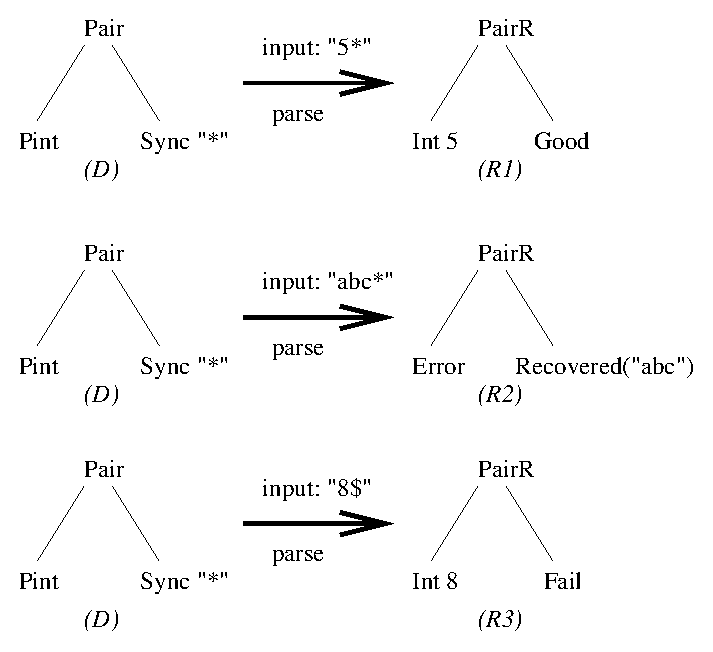
\includegraphics[width=0.8\columnwidth]{parse}
%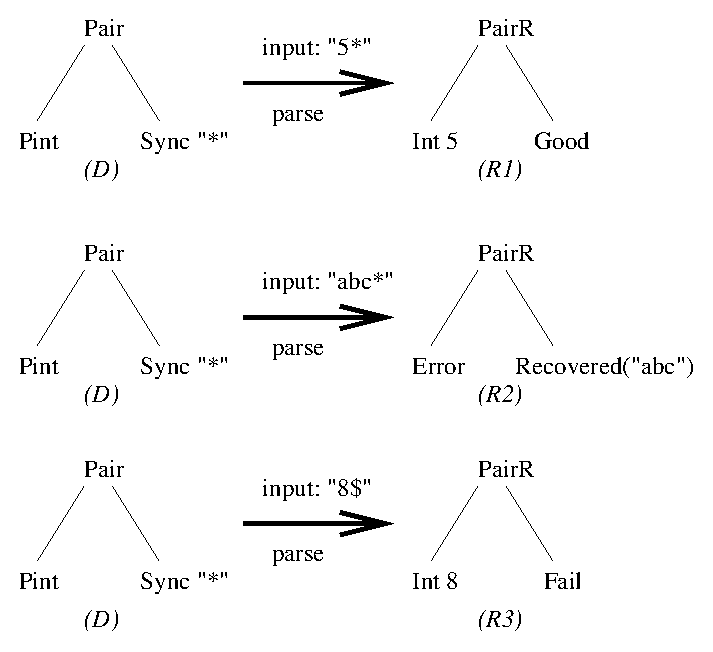
\epsfig{file=parse.eps, width=0.8\columnwidth}
\caption{Result of parsing three input lines}\label{fig:parse}
\end{center}
\end{figure}

\begin{figure*}[t]
\begin{center}
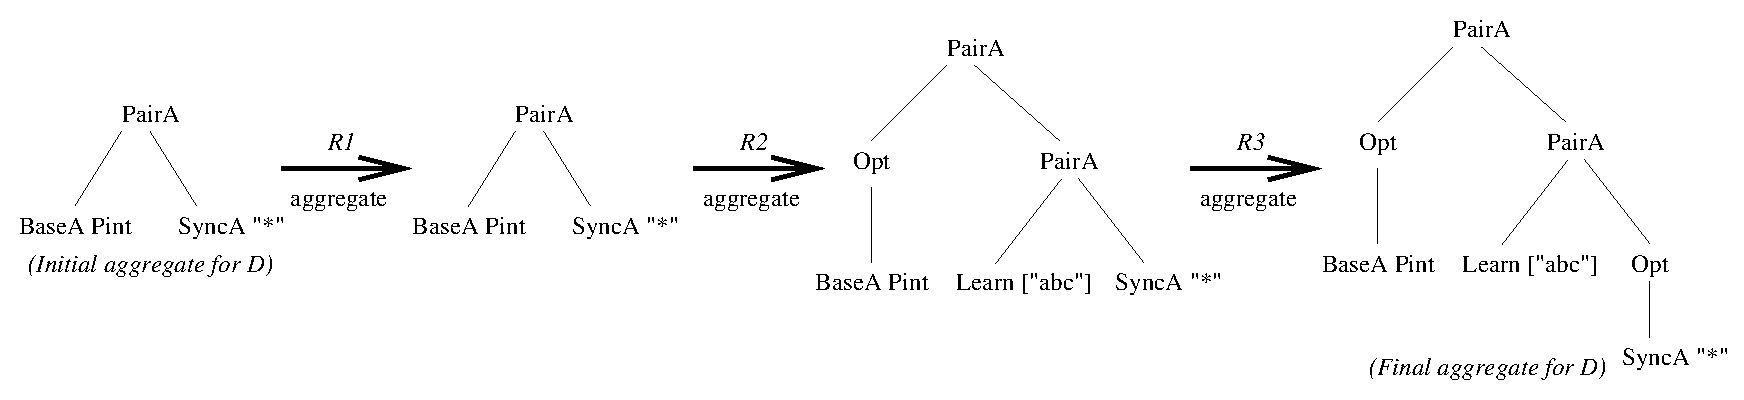
\includegraphics[width=2\columnwidth]{aggregate}
%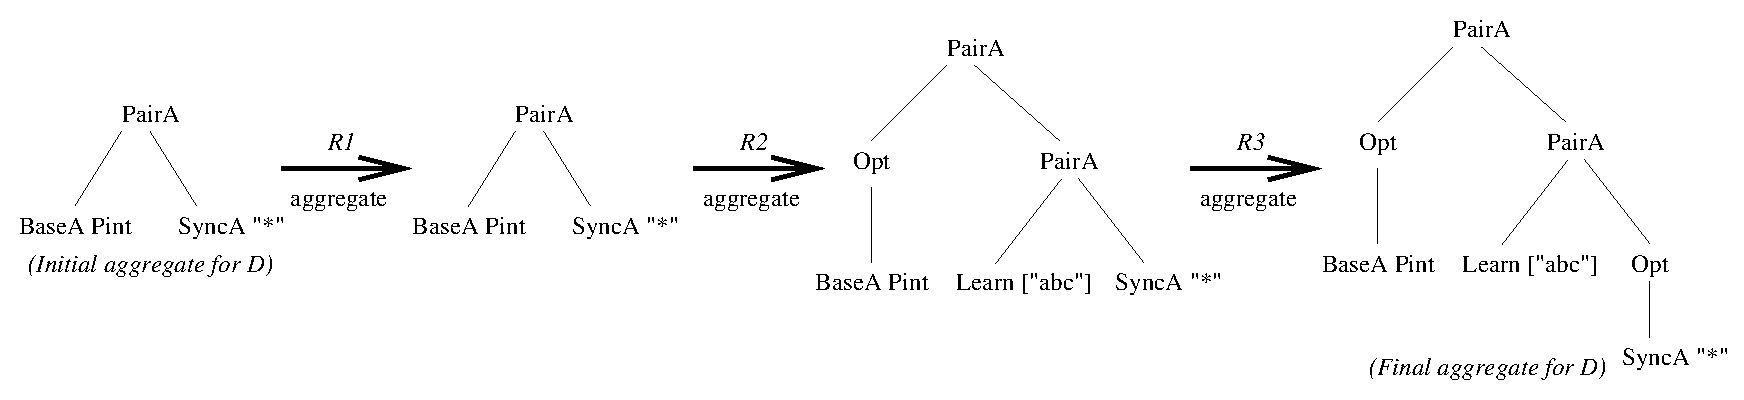
\epsfig{file=aggregate.eps, width=2\columnwidth}
\caption{Aggregation of three parses}\label{fig:aggregate}
\end{center}
\end{figure*}


%\begin{codebox}
%parse_all (d, x) =
%  switch (d) \{
%    case Pint =>  
%      (s, remainder) := match_prefix(x, "[0-9+\-]+");
%      if s != "" then return (Int s, remainder)
%      else return [(Error, x)];
%    case PstringME(re) => 
%      (s, remainder) := match_prefix(x, re);
%      if s != "" then return (Str s, remainder)
%      else return [(Error, x)];
%    case Sync s => 
%      (s', prefix, remainder) := match(x, s);
%      if s' = s and prefix = "" then return (Good, remainder)
%      elseif s' = "" then return (Fail, remainder)
%      else return [(Recovered prefix, remainder)]
%    case (x:d1, d2) =>
%      rs1 := parse_all (d1, x);
%      rs2 := [];
%      foreach (r1, remainder) in rs1 \{
%        (r2, remainder2) := parse_all (d2, remainder);
%        rs2 := rs2 + [((r1, r2), remainder2)]
%      \}
%    case (d1 + d2) => 
%	parse_all(d1, x) @ parse_all(d2, x)
%    case d array(sep, term) =>
%  \} 
%\end{codebox}    
%

\cut{%%%%%%%%%%%%%%%%%%%%%%%%%%%%%%%%

The {\tt parse\_all} function takes a description $d$ and an input string $x$, and returns
a list of all possible parses along with their respective ending position in the input. 
This function implements a standard recursive descent parser which recursively matches the
description structure (and sub-structures) with the input. To parse a pair $x: d_1 * d_2$, 
we first call {\tt parse\_all} on $d_1$ and get a list of parses. 
And then for each of the parse $r_1$ and corresponding end position, we bind $x$ to $r_1$ in
a private environment and  parse $d_2$ to get parses $l_2$. 
Finally for each parse $r_2$ in $l_2$ and each parse $r_1$ in $l_1$, 
construct a representation $(r_1, r_2)$, and return a list of all such pairs.
To parse a union $d_1 + d_2$, we simply return the concatenation of list of parses from
parsing $d_1$ and the list of parses from parsing $d_2$. To parse $d~ array(s, t)$,
we repeatedly attempt to parse $d$ until there's no more progress in the input.
And in each iteration, we also add parses generated from parsing $t$ as well, as if
the array has been terminated at this iteration. Figure \ref{fig:parse_base}
shows the {\tt parse\_base} function which parses a base token. The {\tt match\_prefix}
function matches the prefix of an input string with a regular expression and returns
the matched string and the remainder in the input. The {\tt match} function looks for
the first match of $s$ in input $x$, and returns the matched string $s'$, the prefix string
in $x$ before $s'$, and the remainder in the input.

\begin{figure}[t]
\begin{codebox}
parse_base (b, x) =
  switch (b) \{
  case Pint => 
    (s, suffix) := match_prefix(x, "[0-0+\-]+");
    if s <> "" then return [(Int s, suffix)];
    else return [(Error, x)]
  case PstringME(re) => 
    (s, suffix) := match_prefix(x, re);
    if s <> "" then return [(Str s, suffix)];
    else return [(Error, x)];
  case Sync s => 
    (s', prefix, remainder) := match(x, s);
    if s' = s and prefix = "" then 
      return (Good, remainder)
    elseif s' = "" then 
      return (Fail, remainder)
    else return [(Recovered prefix, remainder)]
  \}
\end{codebox}
\caption{Function to parse a base token or a sync token} \label{fig:parse_base}
\end{figure}

As an example, let $d$ be {\tt (Pint, Sync "|") + (PstringME "[a-z]+", Sync "|")}, 
and $x$ be ``\verb#abc|#''. {\tt parse\_all(d, x)} gives the following two possible parses:
{\small
\begin{verbatim}
  inl (Error, Recovered "abc")
  inr (Str "abc", Good)
\end{verbatim}
}

The {\tt aggregate} function adds a parse into an existing aggregate structure. When there is
no errors in the parse, it makes no changes to the aggregate. If the parse contains 
an error or failure for parsing token $b$, then the aggregate component 
$b$ is transformed to $opt~ b$, to indicate that $b$ node is optional. 
If a parse contains a recovered data $Recovered~ r$, then
a optional learn node will be created before the sync node. And the new aggregate component will be
$(opt (l [r]),~ Sync~ s)$. If the aggregate structure already contains the learn node before this
sync node, then recovered data $r$ will be added to the list under $l$.


}%%%%%%%%%%%%%%%%%%%%%%%%%%%%%%%%% END OF CUT %%%%%%%%%%%%%%%%

% - problem definition (as close to the previous description as possible) (but we don't
%   have a metric to measure how close yet, do we want to mention tree edit distance??)
% - overview of algorithm: parsing + aggregating + rewriting
% - parsing algo (parse rep, score metric, pseudo-code)
% - aggregating algo (in pseudo code)
% - selection of top aggregates
% - update original description
% - rewriting rules (data independent, data dependent, OptsTable)


